% Ground-state convergence against the degrees of freedom, GWW2 isospectral drum:
% the eigenvalue itself on the left, the relative error on the right.
%
% Requires in the preamble:
%   \usepackage{graphicx}
%   \usepackage{subfig}
%   \usepackage{epstopdf}   % the figures are EPS; needed under pdflatex,
%                           % which then wants -shell-escape. Not needed for
%                           % latex/dvips, which reads EPS directly.
%
% The figures live next to this file, in
% results_paper/eigenvalues_convergence/. If you \input this snippet
% from elsewhere, point graphicx at that folder, e.g.
%   \graphicspath{{results_paper/eigenvalues_convergence/}}
% and drop the leading path from the \includegraphics arguments below.

\begin{figure}[htbp]
  \centering
  \subfloat[Eigenvalue $\lambda_1$.\label{fig:convergence_gww2_lambda1_value}]{%
    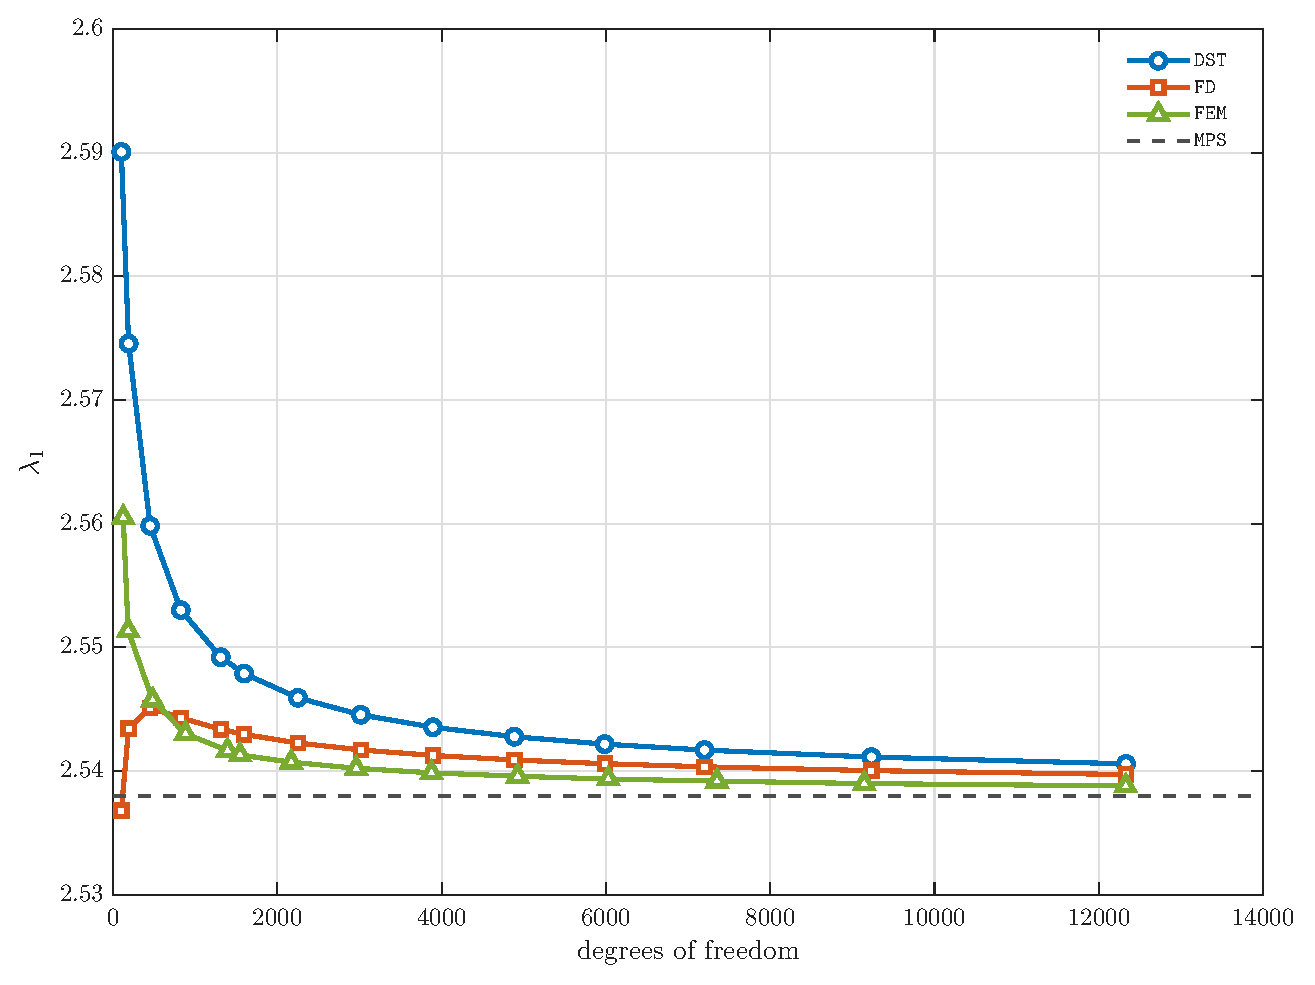
\includegraphics[width=0.45\textwidth]{gww2_convergence_lambda1}}
  \qquad
  \subfloat[Relative error $\frac{|\lambda_1 - \lambda_1^{\text{MPS}}|}{\lambda_1^{\text{MPS}}}$.\label{fig:convergence_gww2_lambda1_error}]{%
    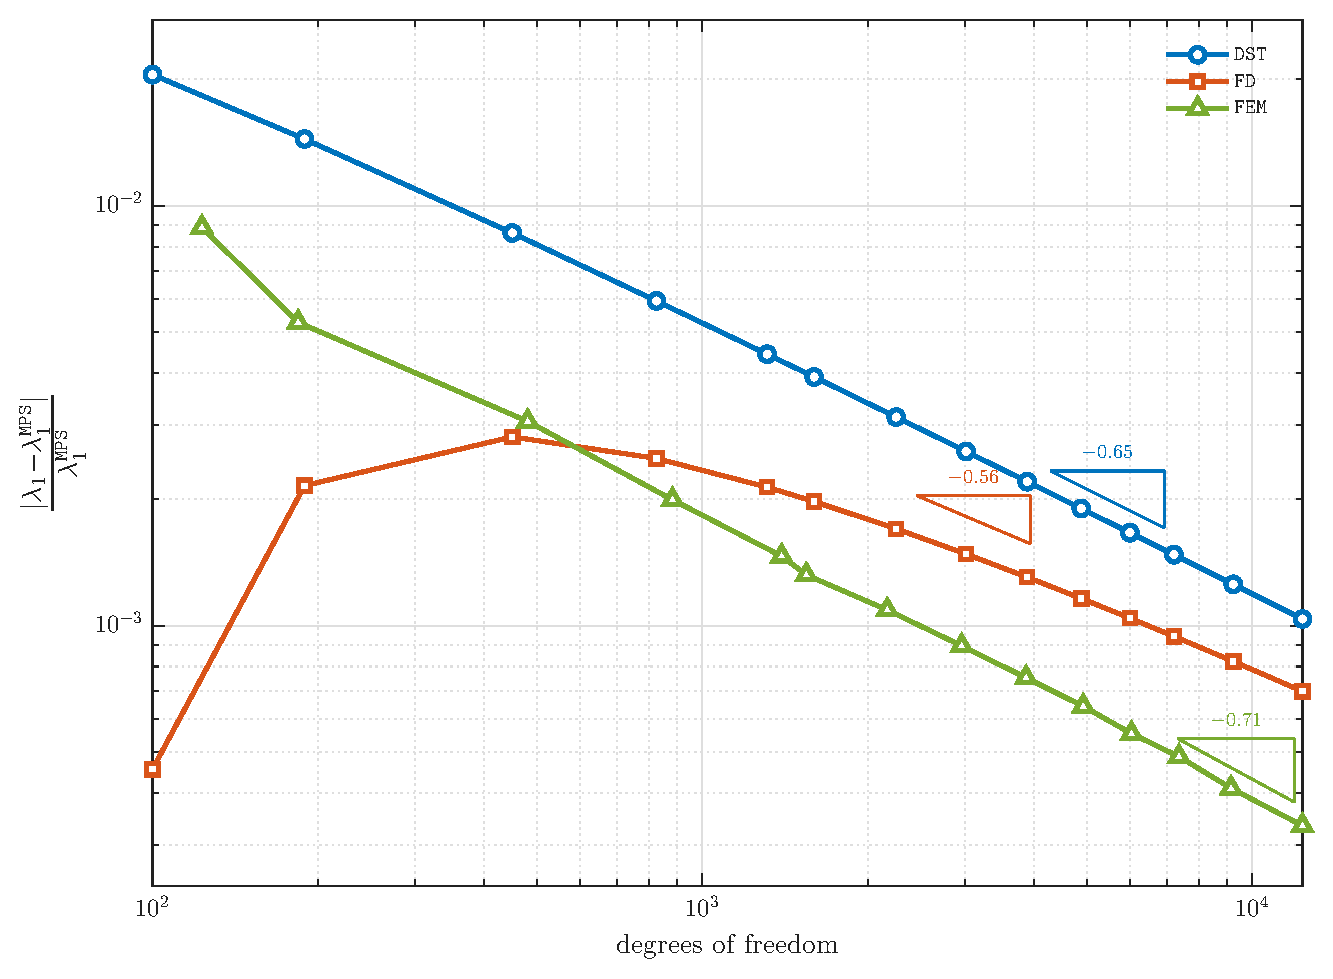
\includegraphics[width=0.45\textwidth]{gww2_convergence_lambda1_error}}
  \caption{The first eigenvalue $\lambda_1$ of Laplace operator, zero Dirichlet boundary conditions, GWW2 isospectral drum \texttt{gww2}. Eigenvalue $\lambda_1$ computed by each discretisation \texttt{DST}, \texttt{FD} and \texttt{FEM} with varying degrees of freedom; compared with the reference eigenvalue $\lambda_1^{\text{MPS}}$ obtained by the method of particular solutions (\texttt{MPS}).}
  \label{fig:convergence_gww2_lambda1}
\end{figure}
